\PassOptionsToPackage{sols}{handout}
\documentclass[main]{subfiles}
\setcounterrefbeforedot{chapter}{m-ws5-2}
\setcounterrefafterdot{section}{m-ws5-2}
\addtocounter{section}{-1}
\usepackage{solutions}

\begin{document}

\ifSubfilesClassLoaded{%
  \chaptermark{\chapterfive}
}{}

\section{The Definite Integral} \label{ws5-2}

\begin{problemonly}
    \begin{framed}

\textbf{Key Ideas}:

\begin{itemize}[topsep=0pt,partopsep=0pt,parsep=8pt,itemsep=0pt]

\item You should recognize and be able to use the notation
  $\displaystyle \int_a^b f(t)\,dt$ for the definite integral. 

\item You should be comfortable thinking about the definite integral
  $\displaystyle \int_a^b f(t)\,dt$ in three ways:
  \begin{itemize}[topsep=0pt]
  \item It can be visualized as a signed area.
  \item If $f$ is a rate function, then $\displaystyle \int_a^b
    f(t)\,dt$ can be interpreted as a net change from $t=a$ to $t=b$.
  \item It is defined as a limit of left-hand sums or right-hand sums.
  \end{itemize}

\item You should be able to use the graphical interpretation of the
  definite integral to evaluate $\displaystyle \int_a^b f(t)\,dt$ when
  $f$ is a function whose graph is simple or has useful symmetry.

\end{itemize}
\end{framed}
\end{problemonly}

\begin{enumerate}
\item 
  \note{This is to reinforce the idea of signed area.  In case you want to
    use the applet to demo this, the formula for $f(t)$ is $2 t^3-19
    t^2+42 t-1$.}

  {%
    \providecommand{\graphcommand}{}
    \renewcommand{\graphcommand}[1]{
      \begin{tikzpicture}[declare function={f(\x) =
          -1+42*\x-19*\x^2+2*\x^3;}]
        \begin{axis}[grid=major, xmax=7.5, xtick={1, 2, ..., 8}, ytick={-16,
            -8, ..., 64}, ymin=-20, ymax=52, xlabel=$t$]
          #1          
          \addplot+[domain=0:8, black] {f(x)};
        \end{axis}
      \end{tikzpicture}
    }      
    The population of a tiny island country changes over time, as people
    immigrate and emigrate.  Suppose $f(t)$ gives the rate of change of
    the population, where $t$ is measured in years. We are interested
    in the next change in population from time $t=1$ to $=7$. 

    \begin{center}
    \begin{tabular}{c}
      {\small $f(t) = $ rate of change of island's population} \\
      {\small (people per year)}  \\
      \graphcommand{
        \solonly{
            \foreach \x in {1,1.5,...,3} {
            \addplot[ybar interval, plusarea] coordinates {(\x,{f(\x)}) 
            (\x+0.5,{f(\x)})};
            }
            \foreach \x in {3.5,4,...,6} {
            \addplot[ybar interval, minusarea] coordinates {(\x,{f(\x)}) 
            (\x+0.5,{f(\x)})};
            }
            \foreach \x in {6.5} {
            \addplot[ybar interval, plusarea] coordinates {(\x,{f(\x)}) 
            (\x+0.5,{f(\x)})};
            }
        }
      } \\
      {\small represent $L_{12}$}
    \end{tabular}
    \end{center}
    
    \begin{enumerate}
    \item
        \note{I'll have half the class do part i and the other half do 
        part ii.}
        
        Let's approximate the net change by
        partitioning the six-year interval into $12$ half-year intervals.
        In these subintervals the rate doesn't change quite as dramatically
        as it does on larger intervals. On each interval we can approximate
        the rate by the rate at the left endpoint of each interval, giving us
        $L_{12}$, or the rate at the right endpoint of each interval, giving
        us $R_{12}$.
        \begin{enumerate}[topsep=0pt]
          \item $L_{12}$ is the sum of 12 terms. Write the first two,
          followed by $+\cdots+$ and then the last term. Sketch a
          visualization of $L_{12}$ on the graph above.
          
          \begin{solution}
              \[\boxed{L_{12}=\tfrac{1}{2}f(1) + \tfrac{1}{2}f(1.5) 
              + \cdots +
              \tfrac{1}{2}f(6.5)}\]
          \end{solution}
          \pspace{\vfill\newpage}

        \begin{center}
        \begin{tabular}{c} 
      {\small $f(t) = $ rate of change of island's population} \\
      {\small (people per year)} \\
      \graphcommand{
        \solonly{
            \foreach \x in {1,1.5,...,2.5} {
            \addplot[ybar interval, plusarea] coordinates {(\x,{f(\x+0.5)}) 
            (\x+0.5,{f(\x+0.5)})};
            }
            \foreach \x in {3,3.5,...,5.5} {
            \addplot[ybar interval, minusarea] coordinates {(\x,{f(\x+0.5)}) 
            (\x+0.5,{f(\x+0.5)})};
            }
            \foreach \x in {6,6.5} {
            \addplot[ybar interval, plusarea] coordinates {(\x,{f(\x+0.5)}) 
            (\x+0.5,{f(\x+0.5)})};
            }
        }
      } \\
      {\small represent $R_{12}$}
    \end{tabular}
    \end{center}
    
          \item $R_{12}$ is the sum of 12 terms. Write the first two,
          followed by $+\cdots+$ and then the last term. Sketch a
          visualization of $R_{12}$ on the graph above.

          \begin{solution}
              \[\boxed{R_{12}=\tfrac{1}{2}f(1.5) + \tfrac{1}{2}f(2) 
              + \cdots +
              \tfrac{1}{2}f(7)}\]
          \end{solution}
          \pspace{24pt}
        \end{enumerate}



    \item Suppose we decided to partition the time interval $[1,7]$ into $24$
    equal sub-intervals. How long would each sub-interval be? What if we
    partitioned $[1,7]$ into $100$ equal sub-intervals? What if we partioned
    into $n$ equal sub-intervals?

    \begin{solution}
        The entire interval $[1,7]$ is $6$ seconds long. If we partitioned
        the interval into $24$ equal sub-intervals, each sub-interval would
        be $6/24=\boxed{0.25 \text{ seconds}}$ long. If we partitioned the
        interval into  $100$ equal sub-intervals, each sub-interval would be
        $6/100=\boxed{0.06\text{ seconds}}$ long. If we partitioned the
        interval into $n$ equal sub-intervals, each sub-interval would be
        $\boxed{6/n \text{ seconds}}$ long.
    \end{solution} 
    \pspace{\vfill}

    \item
      \begin{problem}[24pt]
        How would you visualize the \emph{exact} net change in population
        between $t = 1$ and $t = 7$?
      \end{problem}

      \begin{solution}
        We can visualize the exact net change in population between $t =
        1$ and $t = 7$ as the signed area between the curve and the
        $x$-axis.  That's the area of the green regions below minus the
        area of the red region:
        \begin{center}
          \graphcommand{%
            \addplot+[plusarea, domain=1:3.44] {f(x)} \closedcycle; %
            \addplot+[minusarea, domain=3.44:6.03] {f(x)} \closedcycle; %
            \addplot+[plusarea, domain=6.03:7] {f(x)} \closedcycle; %
          }          
        \end{center}
      \end{solution}

      \begin{problemonly}
        \begin{framed}
          \textbf{Notation.} We write this quantity as $\displaystyle
          \int_1^7 f(t)\,dt$.  The variable $t$ here is a ``dummy
          variable'', so we could also write it as $\displaystyle \int_1^7
          f(x)\,dx$ (or use any other letter in place of $t$ without
          changing the meaning).  We read this as \uline{the definite
            integral of $f$ from $1$ to $7$}.
        \end{framed}
      \end{problemonly}

      

    \item
      \begin{problem}[\vfill]
        Was the population larger at time $t = 1$ or time $t = 7$?  How do
        you know?
      \end{problem}

      \begin{solution}
        From our picture in
        {{{{\#1}}(b)}},
        we can see that the net change from $t = 1$ to $t = 7$ is
        positive; therefore, the population was larger at \fbox{$t = 7$}.
      \end{solution}

    \item

      \note{Students often have trouble with the difference between ``net
        change'' and ``amount.''}

      \begin{problem}[\vfill]
        Suppose the population at time $t = 2$ was $2000$ people.
        Write an expression involving a definite integral which gives the
        number of people at time $t = 4$.
      \end{problem}

      \begin{solution}
        Definite integrals always tell us about net change, so let's first
        find the net change between $t = 2$ (when we know the population)
        and $t = 4$: that's $\displaystyle \int_2^4 f(t)\,dt$.  As an
        equation, we've just said
        \begin{align*}
          \text{(population at $t = 4$)} - \text{(population at $t = 2$)}
          &= \int_2^4 f(t)\,dt, \\
          \shortintertext{so} %
          \text{(population at $t = 4$)} &= \text{(population at $t = 2$)}
          +
          \int_2^4 f(t)\,dt \\
          &= \boxed{2000 + \int_2^4 f(t)\,dt}
        \end{align*}
      \end{solution}

    \end{enumerate}  
  }

\end{enumerate}

\pspace{\newpage}

\begin{framed}
  \textbf{The Definite Integral.}  We have three major ways of thinking
  about the definite integral $\displaystyle \int_a^b f(x)\,dx$:
  \begin{enumerate}[itemsep=8pt]
  \item If $a < b$, we visualize it as: \fitb{4in}{the signed area under $f$
      from $a$ to $b$}

    \begin{center}
      \begin{tikzpicture}[declare function={f(\x) = \x * (\x - 2) * (\x + 0.8) + 0.5;}]
        \begin{axis}[xtick={-1.4, 1.25}, xticklabels={$a$, $b$}, hide y
          axis, width=2.5in, clip=false]
          \solonly{
            \addplot+[domain=-1.4:-0.973, minusarea] {f(x)} \closedcycle;
            \addplot+[domain=-0.973:0.27, plusarea] {f(x)} \closedcycle;
            \addplot+[domain=0.27:1.25, minusarea] {f(x)} \closedcycle;
          }
          \addplot+[domain=-1.45:2.15, black] {f(x)}
          node[right] {$y = f(x)$};
        \end{axis}
      \end{tikzpicture}
    \end{center}

  \item If $f$ is a rate function, then we interpret $\displaystyle
    \int_a^b f(x)\,dx$ as \fitb{2in}{the net change from $x = a$
      to $x = b$}

  \item $\displaystyle \int_a^b f(x)\,dx$ is actually defined to be
    $\fitb{3in}{\displaystyle \lim_{n \to \infty} R_n \text{ \textbf{or}
      } \lim_{n \to \infty} L_n}$

  \end{enumerate}
\end{framed}

\begin{enumerate}[resume]
\item 
  \begin{enumerate}
  \item

    \note{This is to help students get used to the notation and to see
      that they can compute certain definite integrals using geometry.
      
      Matt note - this is something to repeatedly emphasize throughout the unit, as they will often forget this is an option later.} 

    \begin{problem}[\vfill]
      Evaluate $\displaystyle \int_{-1}^2 (|t| - 1)\,dt$. 
    \end{problem}

    \begin{solution}
      Graphically, this is the signed area under $y = |t| - 1$ from $t =
      -1$ to $t = 2$, pictured below:
      \begin{center}
        \begin{tikzpicture}
          \begin{axis}[width=3in, axis equal=true, xlabel=$t$];
            \addplot+[minusarea, domain=-1:1] {abs(x) - 1} \closedcycle;
            \addplot+[plusarea, domain=1:2] {abs(x) - 1} \closedcycle;
            \addplot+[domain=-1.5:2.5, black] {abs(x) - 1} node[pos=1,
            left] {$|t| - 1$};
          \end{axis}
        \end{tikzpicture}
      \end{center}
      The red region is a triangle of width 2 and height 1, so its area is
      $\frac{1}{2}(2)(1) = 1$; the green region is a triangle of width 1
      and height 1, so its area is $\frac{1}{2} (1)(1) = \frac{1}{2}$.
      Therefore, $\displaystyle \int_{-1}^2 (|t| - 1)\,dt = -1 +
      \frac{1}{2} = \boxed{-\frac{1}{2}}$.
    \end{solution}

  \item Suppose $|t| - 1$ gives the rate (in gallons per hour) of water
    flowing into and out of a tank $t$ hours after noon on a particular
    day.  Which of the following is a correct interpretation of
    $\displaystyle \int_{-1}^2 (|t| - 1)\,dt$?
    \begin{enumerate}[label=\protect\maybecircle{\Alph*.},ref=\Alph*]
    \plainitem It is the amount of water in the tank at 2 pm.
    \plainitem It is the amount of water in the tank at 11 am.
    \circleitem It is (amount of water in the tank at 2 pm) $-$ (amount of
      water in the tank at 11 am).
    \plainitem It is (amount of water in the tank at 11 am) $-$ (amount of
      water in the tank at 2 pm).
    \end{enumerate}

    \pspace{\nstretch{0.25}}

  \end{enumerate}

\item 
  \raisebox{2ex-\height}{
    \begin{minipage}[t]{2.5in}
      \vspace{0pt}
      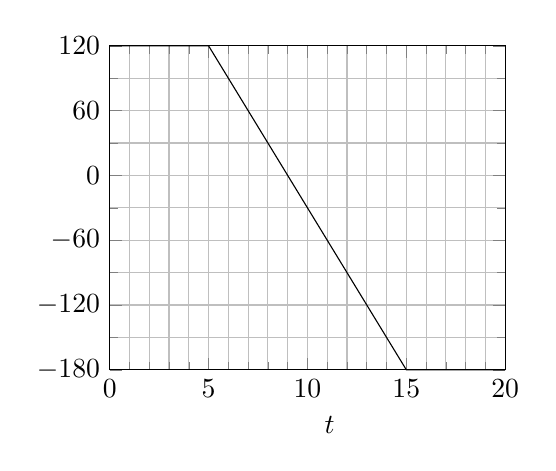
\begin{tikzpicture}
        \begin{axis}[cycle list=black, ytick={-180, -120, ..., 120},
          enlargelimits=false, clip=false, grid=major, width=2.6in, axis
          line style={shorten >=-8pt, shorten <=-8pt}, xlabel
          style={xshift=8pt}, xlabel=$t$, minor xtick={1,
              2, ..., 20}, minor ytick={-150, -90, ..., 90}, grid=both]
          \addplot+[sharp plot] coordinates { (0, 120) (5, 120) (15,
            -180) (20, -180) };
        \end{axis}
      \end{tikzpicture}
    \end{minipage}
  }
  \hspace{0.1in}
  \begin{minipage}[t]{\linewidth-2.6in-15pt}
    \vspace{0pt} The function $r(t)$ graphed to the left gives the rate at
    which water is flowing into or out of a backyard swimming pool. Time
    $t$ is measured in hours, and the rate $r(t)$ is measured in gallons
    per hour.  At time $t=0$, there are 700 gallons of water in the pool.
  \end{minipage}

  \begin{enumerate}
  \item
    \begin{problem}[0.3in]
      Write a definite integral that represents the net change in the
      amount of water in the pool from time $t=0$ to $t=6$ hours, and find
      this net change exactly.  
    \end{problem}

    \begin{solution}
      The net change in the amount of water in the pool from time $t=0$ to
      $t=6$ is $\boxed{ \int_0^6 r(t)\,dt}$.  This is the area under the
      graph of $r(t)$ from $t = 0$ to $t = 6$, which is $\boxed{705}$.
    \end{solution} 

  \item
    \begin{problem}
      How much water is in the pool at time $t=6$?
    \end{problem}

    \begin{solution}
      In {{{{\#3}}(a)}}, we found
      that the pool gains $705$ gallons of water between $t = 0$ and $t =
      6$.  We were told that the pool had 700 gallons of water at $t = 0$,
      so at $t = 6$, it has $700 + 705 = \boxed{1405}$ gallons of water.
    \end{solution}

  \item
    \begin{problem}[0.25in]
      When is water entering the pool at the greatest rate?  What is this
      greatest rate?
    \end{problem}

    \begin{solution}
      We're looking for when the rate graph is highest, which happens
      \fbox{from $t = 0$ to $t = 5$}; the rate during this time is
      \fbox{120 gallons per hour}.
    \end{solution}

  \item
    \begin{problem}[\vfill]
      When is the amount of water in the pool greatest?  At that time,
      how much water is in the pool?
    \end{problem}

    \begin{solution}
      From $t = 0$ to $t = 9$, the pool is gaining water; from $t = 9$
      to $t = 20$, it's losing water.  Therefore, the amount of water in
      the pool must be greatest at \fbox{$t = 9$}.  Moreover,
      \begin{align*}
        \text{(amount of water in pool at $t = 9$)} &= \text{(amount of
          water in pool at $t = 0$)} + \int_0^9 r(t)\,dt \\
        &= 700 + (\text{area under graph of $r(t)$ from $t = 0$ to $t =
          9$}) \\
        &= 700 + 840 \\
        &= \boxed{1540 \text{ gallons}}
      \end{align*}
    \end{solution}

  \item

    \note{The point here is to make sure students understand that we can
      write just a single integral from 4 to 12; we don't need to split it
      up into when the rate is positive and when it's negative.}

    \begin{problem}[0.25in]
      Between $t=4$ and $t=12$, what is the net change in the amount of
      water in the pool?  Express your answer as a definite integral.
    \end{problem}

    \begin{solution}
      $\displaystyle \int_4^{12} r(t)\,dt$.
    \end{solution}

  \item
    \begin{problem}[\stretch{1.5}]
      Recall that, at $t=0$, the pool contains 700 gallons of water. Is
      there ever another time $T$ at which the pool contains 700 gallons
      of water?  If so, what is $T$?  If not, why not?
    \end{problem}

    \begin{solution}
      As we saw in {{{{\#3}}(d)}}, the
      pool starts out with 700 gallons of water and has gained an
      additional 840 gallons by $t = 9$.  After this, the pool starts
      losing water.  We can see that, by $t = 20$, it has lost more
      water than it gained, so there must have been some time before $t
      = 20$ when it had exactly 700 gallons.  Graphically, we're looking
      for the time $T$ when the signed area from $t = 0$ to $t = T$ is
      exactly 0:
      \begin{center}
        \begin{tikzpicture}
          \begin{axis}[cycle list=black, ytick={-180, -120, ..., 120},
            enlargelimits=false, clip=false, grid=major, width=2.6in, axis
            line style={shorten >=-8pt, shorten <=-8pt}, xlabel
            style={xshift=8pt}, xlabel=$t$, minor xtick={1,
                2, ..., 20}, minor ytick={-150, -90, ..., 90},
              grid=both, extra x ticks={16.67}, extra x tick
            labels={$T$}, extra x tick style={grid=none}]
            \addplot+[sharp plot, plusarea] coordinates {(0, 120) (5,
              120) (9, 0)} \closedcycle;
            \addplot+[sharp plot, minusarea] coordinates { (9, 0) (15,
              -180) (16.67, -180) } \closedcycle;
            \addplot+[sharp plot] coordinates { (0, 120) (5, 120) (15,
              -180) (20, -180) };
          \end{axis}
        \end{tikzpicture}          
      \end{center}
      That is, the area of the red region must be exactly the same as
      the area of the green region, which is 840.  The portion of the
      red region from $t = 9$ to $t = 15$ is a triangle of width $6$ and
      height $180$, so it has area $\frac{1}{2} \cdot 6 \cdot 180 =
      540$.  Therefore, we want the portion of the red region from $t =
      15$ to $t = T$ to have area $840 - 540 = 300$.  This portion is a
      rectangle of height $180$, so its width must be $\frac{300}{180} =
      \frac{5}{3}$.  Therefore, $\displaystyle T = 15 + \frac{5}{3} =
      \boxed{\frac{50}{3}}$. 
    \end{solution}

  \item
    \begin{problem}[\stretch{2}]
      Let $W(t)$ be the amount of water in the pool at time $t$.  Sketch a
      rough graph of $W(t)$, and make sure your graph agrees with your
      answers to the previous parts of this problem. 
    \end{problem}

    \begin{solution}
      We are told that, at time $t = 0$, the pool has 700 gallons per
      water.  From $t = 0$ to $t = 5$, it gains water at a constant rate
      of 120 gallons per hour, so $W(t)$ will be linear on $[0, 5]$ with
      slope 120.

      From $t = 5$ to $t = 9$, the amount of water continues increasing,
      but at a decreasing rate.  Therefore, $W(t)$ is increasing and
      concave down on this interval.  Moreover, we know that $W(t)$
      reaches its maximum value of $1540$ at $t = 9$.

      From $t = 9$ to $t = 15$, the amount of water is decreasing, and it
      decreases at a faster rate as time goes on.  Therefore, $W(t)$ is
      decreasing and concave down on this interval.

      From $t = 15$ to $t = 20$, the amount of water decreases at a
      constant rate of 180 gallons per hour, so $W(t)$ will be linear on
      $[15, 20]$ with slope $-180$.

      We can also use our work in the previous parts to label a few
      additional points on the graph.  In
      {{{{\#3}}(b)}}, we found that
      there are 1405 gallons of water in the pool at $t = 6$.  In
      {{{{\#3}}(f)}}, we found that the pool has
      700 gallons of water at $t = \frac{50}{3}$.  

      Putting all of this together, we get the following graph:
      \begin{center}
        \begin{tikzpicture}
          \begin{axis}[ytick={700, 1540}, enlargelimits=true, clip=false,
            width=3.5in, height=2.5in, xlabel=$t$, ymin=0]
            \addplot+[domain=0:5] {120*x + 700} node[pos=0.5,
            pin=-80:{slope 120}] {}; %
            \addplot+[domain=5:9] {-15 * (x^2 - 18*x + 25) + 700}; %
            \addplot+[domain=9:15] {-15 * (x^2 - 18*x + 25) + 700}; %
            \addplot+[domain=15:20] {3700 - 180 * x} node[pos=0.5,
            pin=-100:{slope $-180$}] {}; %
            \addplot+[black, closed] coordinates { (6, 1405) (9, 1540)
              (16.67, 700) } node[pos=0, anchor=south east, inner sep=1pt]
            {$(6, 1405)$} node[pos=0.5, above] {$(9, 1540)$} node[pos=1,
            anchor=south west, inner sep=1pt] {$\left( \frac{50}{3}, 700
              \right)$}; 
          \end{axis}
        \end{tikzpicture}          
      \end{center}
      \checkmark\ 
        Notice that this agrees with our work in the previous parts:
        \begin{itemize}[nosep]
        \item In {{{{\#3}}(c)}}, we said
          water was entering the pool at the greatest rate between $t = 0$
          and $t = 5$.  That is reflected in our graph of $W(t)$ by the
          fact that the slope of $W(t)$ is most positive between $t = 0$
          and $t = 5$.
        \item In {{{{\#3}}(d)}}, we said
          the amount of water in the pool is greatest at $t = 9$.  That is
          reflected in our graph of $W(t)$ by the fact that the graph has
          its absolute maximum at $t = 9$.
        \end{itemize}
    \end{solution}

  \item \note{Just to make sure they are comfortable visualizing definite
      integrals as signed area.}

    \begin{problem}[\nstretch{0.1}]
      Put the following quantities in increasing order: $\displaystyle
      \int_5^8 r(t)\,dt \quad \int_5^9 r(t)\,dt \quad \int_5^{10}
      r(t)\,dt \quad \int_5^{11} r(t)\,dt$.
    \end{problem}

    \begin{solution}
      By visualizing these as signed areas, we see that
      \[\boxed{\int_5^{11} r(t)\,dt < \int_5^8 r(t)\,dt= \int_5^{10}
        r(t)\,dt < \int_5^9 r(t)\,dt}.\]
    \end{solution}

  \end{enumerate}

\item 
  \begin{problem}[4in]
    Let $f$ be a differentiable function, such that $f>0$ and $f'>0$ on
    $[2, 12]$.  Suppose we approximate $\displaystyle \int_2^{12} f(x)\,dx$
    using left-hand and right-hand sums $L_n$ and $R_n$ for different
    values of $n$.

    Put the following expressions in increasing order:
    \[ \int_2^{12} f(x)\,dx \qquad L_{10} \qquad L_{20} \qquad L_{100}
    \qquad R_{30} \qquad R_{60}.\] (Some sketches will help!)
  \end{problem}

  \begin{solution}
    Since $f$ is increasing, left-hand sums will be underestimates for
    $\displaystyle \int_2^{12} f(x)\,dx$, and right-hand sums will be
    overestimates.  To get some idea of how to compare $L_{10}$, $L_{20}$,
    and $L_{100}$, let's look at a simpler example, $L_5$ vs. $L_{10}$:
    \begin{center}
      \begin{tikzpicture}[declare function={f(\x) = 2^(\x/6) + 2;}]
        \begin{axis}[hide y axis, xtick={2, 12}, ymin=0, width=2.5in,
          clip=false]
          \addplot+[domain=1:13] {f(x)};
          \addplot+[ybar interval, plusarea] coordinates {
            (2, {f(2)}) (4, {f(4)}) (6, {f(6)}) (8, {f(8)}) (10, {f(10)})
            (12, {f(10)})
          };
          \draw (axis cs: -2, 3) node { $L_5$: };
        \end{axis}
      \end{tikzpicture}

      \begin{tikzpicture}[declare function={f(\x) = 2^(\x/6) + 2;}]
        \begin{axis}[hide y axis, xtick={2, 12}, ymin=0, width=2.5in,
          clip=false] 
          \addplot+[domain=1:13] {f(x)}; %
          \addplot+[ybar interval, plusarea] coordinates { %
            (2, {f(2)}) (3, {f(3)}) (4, {f(4)}) (5, {f(5)})
            (6, {f(6)}) (7, {f(7)}) (8, {f(8)}) (9, {f(9)}) (10, {f(10)})
            (11, {f(11)}) (12, {f(11)}) %
          };
          \draw (axis cs: -2, 3) node { $L_{10}$: };
        \end{axis}        
      \end{tikzpicture}
    \end{center}
    As we can see, $L_{10}$ is closer to the actual value of
    $\displaystyle \int_2^{12} f(x)\,dx$, which makes sense since we
    expect that using more rectangles gives us better approximations.
    Therefore, among $L_{10}$, $L_{20}$, and $L_{100}$, the one that is
    closest to $\displaystyle \int_2^{12} f(x)\,dx$ is $L_{100}$, followed
    by $L_{20}$, and finally $L_{10}$.  The idea is the same for $R_{30}$
    and $R_{60}$: $R_{60}$ is closer to $\displaystyle \int_2^{12}
    f(x)\,dx$ than $R_{30}$.  This gives us the ordering 
    \[
    \boxed{ L_{10} < L_{20}<L_{100}< \int_2^{12} f(x)\,dx <R_{60} <
      R_{30}} \]
  \end{solution}

\end{enumerate}

\end{document}
